\documentclass[pdf,aspectratio=169,10pt]{beamer}
\usetheme{%
%Berlin%
%Antibes%
%Boadilla%
%Copenhagen%
%Darmstadt%
%Frankfurt%
%Ilmenau%
%JuanLesPins%
%Madrid%
%Warsaw%
%Marburg%
%Boadilla%
simple%
}


%\usepackage{pgfpages}
%\pgfpagesuselayout{4 on 1}[a4paper,border shrink=5mm]
%\usepackage{scalefnt}
%\usepackage[version=4]{mhchem}
%\newcommand{\bftab}{\fontseries{b}\selectfont}
\usepackage{multirow}
\newcommand{\rot}[1]{\multirow{9}{*}{\rotatebox[origin=c]{90}{#1}}}
%\mode<presentation>


%\usecolortheme[RGB={15,90,0}]{structure}
%\usecolortheme[RGB={20,100,0}]{structure}
%\usecolortheme[RGB={10,80,0}]{structure}

\useinnertheme{circles}
%\useoutertheme{miniframes}
%\useoutertheme{shadow}
%\useoutertheme[subsection=false]{smoothbars}
%\useoutertheme{infolines}

% \usepackage[brazil]{babel}
%\usepackage[T1]{fontenc}
%\usepackage{ae} 
\usepackage[utf8]{inputenc} 
\usepackage[T1]{fontenc}


\usepackage{media9}      

\usepackage[onecol]{hackthefootline}
%\htfconfig{title=short, framenrs=counter, atsep=space}
\usepackage{algorithm}
\usepackage{algorithmic}
\usepackage{graphics}
\usepackage{graphicx}
%\usepackage[caption=false]{subfig}
\usepackage{caption}
%\usepackage{subcaption}
\usepackage{array} %for vertical thick lines in tables
\usepackage{multirow} %multirow tables
\usepackage{nicefrac} %for fractions like 1/4
\usepackage{booktabs}
\usepackage{multicol}
\usepackage{amssymb}
\usepackage{amsmath} 
\usepackage[makeroom]{cancel}
\usepackage{bm}
\usepackage[group-separator={,},separate-uncertainty]{siunitx}
\usepackage[most]{tcolorbox}
\usepackage{xcolor}
\usepackage[export]{adjustbox}

%\usefonttheme[onlymath]{serif}
%\usepackage{lmodern}
\usepackage{makecell}
%% Commande TikZ
\usepackage{tikz}
\usepackage{tikz,pgf,tikz-3dplot}
\usepackage{pgfplots}
\pgfplotsset{compat=1.16}
\usepackage[beamer]{hf-tikz}
\usetikzlibrary{bayesnet,shapes,arrows,positioning}
\tikzstyle{arrow} = [thick,->,>=stealth]
\tikzset{
	%Define standard arrow tip
	>=stealth',
	%Define style for boxes
	punkt/.style={
		rectangle,
		rounded corners,
		draw=black, very thick,
		text width=6.5em,
		minimum height=2em,
		text centered},
	% Define arrow style
	pil/.style={
		->,
		thick,
		shorten <=2pt,
		shorten >=2pt,}
}


\tikzstyle{rempliRed}=[red!30, fill=red!30]
\tikzstyle{ecritRed}=[red!60, fill=red!60]
\tikzstyle{rempliBlue}=[blue!30, fill=blue!30]
\tikzstyle{ecritBlue}=[blue!60, fill=blue!60]

\definecolor{color1}{rgb}{0.25, 0, 0.75}
\definecolor{color2}{rgb}{0.5, 0, 0.5}
\definecolor{color3}{rgb}{0.75, 0, 0.25}

\pgfplotsset{
    dirac/.style={
        mark=triangle*,
        mark options={scale=2},
        ycomb,
        scatter,
        visualization depends on={y/abs(y)-1 \as \sign},
        scatter/@pre marker code/.code={\scope[rotate=90*\sign,yshift=-2pt]}
    }
}

\def\mathunderline#1#2{\color{#1}\underline{{\color{black}#2}}\color{black}}

\DeclareMathOperator{\Tr}{\mathrm{Tr}}
\DeclareMathOperator{\KL}{\mathrm{KL}}
\usepackage{dsfont}


\newcommand{\E}[2][]{
   \ifthenelse{ \equal{#1}{} }
      {\ensuremath{\left\langle#2\right\rangle}}
      {\ensuremath{\left\langle#2\right\rangle_{#1}}}
}

\newcommand{\cov}[2][]{
    \ifthenelse{ \equal{#1}{} }
        {\operatorname{cov}\parens*{#2}}
        {\operatorname{cov}_{#1}\parens*{#2}}
}

%Felipe's packages


% Definitions
\newcommand*{\defeq}{\stackrel{\text{def}}{=}}
\newcommand{\tr}[1]{\operatorname{tr}\left(#1\right)}

\newcommand{\MOGP}{\ensuremath{\mathcal{MOGP}}}
\renewcommand{\L}{{\mathbb L}}
\def\data{\text{data}}
\def\sn{\sigma_{\text{noise}}}
\def\eye{\mathbf{I}}
\def\cN{{\mathcal{N}}}
\def\cX{{\mathcal{X}}}
\def\cY{{\mathcal{Y}}}
\def\dxi{{\text d} \xi}
\def\N{{\mathbb{N}}}
\def\m{{\mathbf{m}}}
\def\NLL{{\text{NLL}}}
\newcommand{\eps}{\varepsilon}
\def\R{{\mathbb{R}}}
\def\MVN{{\text{MVN}}}
\def\GP{{\mathcal {GP}}}
\def\y{{\mathbf{y}}}
\DeclareMathOperator{\OT}{OT}
\def\t{{\mathbf{t}}}
\def\x{{\mathbf{x}}}
\def\xizi{ \xi_0^{(i)} }
\def\u{{\mathbf{u}}}
\def\z{{\mathbf{z}}}
\def\X{{\mathbf{X}}}
\def\K{{\mathbf{K}}}
\def\dtau{{\text d\tau}}
\def\td{{\text d}}
\newcommand{\id}{\text{id}}



\newcommand{\fourier}[1]{\mathcal{F} \left\{#1\right\}}
\newcommand{\WF}[2]{\operatorname{WF}\left([#1],[#2]\right)}

\newcommand{\afourier}[1]{\mathcal{F}^{-1} \left\{#1\right\}}
\newcommand{\srp}[4]{\operatorname{simrect}_{#1,#2,#3}\left(#4\right)}
\newcommand{\rect}[1]{\text{rect}\left(#1\right)}
\def\sinc{ \operatorname{sinc} }
\newcommand{\SK}[1]{\operatorname{SK}\left(#1\right)}
\newcommand{\V}[2]{\mathbb{V}\left[#1,#2\right]}
\newcommand\eqdef{\overset{\mathrm{def}}{=}}
\newcommand{\GSK}[1]{\operatorname{GSK}\left(#1\right)}
\newcommand{\GSKN}[1]{\operatorname{GSK}_N\left(#1\right)}
\DeclareMathOperator\supp{supp}
\def\argmin{\mathop{\rm arg \; min}\limits}%
\def\diag{\mathop{\rm diag}\nolimits}%
%\let\leq=\leqslant
%\let\geq=\geqslant
%colours
\definecolor{navy}{HTML}{000080}
\providecommand{\rbullet}{{\textcolor{red}{{\bf \bullet}}}}
\providecommand{\bbullet}{{\textcolor{navy}{{\bf \bullet}}}}
\definecolor{clay}{RGB}{190,22,34}%
\providecommand{\bred}[1]{\textcolor{clay}{{\bf#1}}}
\providecommand{\bgreen}[1]{\textcolor{green}{{\bf#1}}}
\providecommand{\bteal}[1]{\textcolor{teal}{{\bf#1}}}
\providecommand{\bblue}[1]{\textcolor{navy}{{\bf#1}}}
\providecommand{\red}[1]{\textcolor{clay}{#1}}
\providecommand{\blue}[1]{\textcolor{navy}{#1}}
\providecommand{\bbullet}{{\textcolor{navy}{{\bf \bullet}}}}




%% Commande TikZ
\tikzstyle{rempliRed}=[red!30, fill=red!30]
\tikzstyle{ecritRed}=[red!60, fill=red!60]
\tikzstyle{rempliBlue}=[blue!30, fill=blue!30]
\tikzstyle{ecritBlue}=[blue!60, fill=blue!60]

\newcommand{\er}[1]{{\color{red!60} #1}}
\newcommand{\eb}[1]{{\color{blue!60} #1}}


% Commandes
\newcommand{\bigslant}[2]{{\raisebox{.2em}{$#1$}\left/\raisebox{-.2em}{$#2$}\right.}} 
\newcommand{\Z}{{\mathbb Z}}
\renewcommand{\P}{{\mathbb P}}
\newcommand{\G}{{\mathbb G}}
\renewcommand{\L}{{\mathbb L}}
\newcommand{\T}{{\mathbb T}}
\newcommand{\Q}{{\mathbb Q}}


\newcommand{\PP}{{\mathcal P}}
\newcommand{\HH}{{\mathcal H}}
\newcommand{\DD}{{\mathcal D}}
\newcommand{\BB}{{\mathcal B}}
\newcommand{\MM}{{\mathcal M}}
\newcommand{\XX}{{\mathcal X}}
\newcommand{\YY}{{\mathcal Y}}
\newcommand{\NN}{{\mathcal N}}
\newcommand{\LL}{{\mathcal L}}
\newcommand{\1}{{\mathds 1}}

\newcommand{\bX}{\boldsymbol{X}}
\newcommand{\bY}{\boldsymbol{Y}}
\newcommand{\bnu}{\boldsymbol{\nu}}
\newcommand{\bmu}{\boldsymbol{\mu}}
\newcommand{\boldeta}{\boldsymbol{\eta}}
\newcommand{\bsigma}{\boldsymbol{\sigma}}
\newcommand{\balpha}{\boldsymbol{\alpha}}
\newcommand{\bfun}{\boldsymbol{f}}
\newcommand{\bGamma}{\boldsymbol{\Gamma}}
\newcommand{\br}{\boldsymbol{r}}
\newcommand{\bq}{\boldsymbol{q}}
\newcommand{\bG}{\boldsymbol{G}}
\newcommand{\tH}{\tilde{H}}
\newcommand{\tg}{\tilde{g}}
\newcommand{\tS}{\tilde{\Sigma}}
\def\d{{\text d}}
\def\ba{ \boldsymbol{a} }
\def\bb{ \boldsymbol{b} }
\def\bx{ \boldsymbol{x} }
\def\by{ \boldsymbol{y} }




\newcommand{\CB}[1]{{\color{blue} #1}}
\newcommand{\CR}[1]{{\color{red} #1}}
\newcommand{\CV}[1]{{\color{green} #1}}
\newcommand{\CVI}[1]{{\color{violet} #1}}
\newcommand{\CP}[1]{{\color{purple} #1}}
\newcommand{\CO}[1]{{\color{orange} #1}}
\newcommand{\CM}[1]{{\color{magenta} #1}}
\newtheorem{proposition}{Proposition}  
\newtheorem{remark}{Remark}  



%imports
\usepackage[export]{adjustbox}
\usepackage[absolute,overlay]{textpos}
\setlength{\TPHorizModule}{\textwidth}
\setlength{\TPVertModule}{\textwidth}
\usepackage{soul}

% Pausing in the align environment
\makeatletter
\let\save@measuring@true\measuring@true
\def\measuring@true{%
  \save@measuring@true
  \def\beamer@sortzero##1{\beamer@ifnextcharospec{\beamer@sortzeroread{##1}}{}}%
  \def\beamer@sortzeroread##1<##2>{}%
  \def\beamer@finalnospec{}%
}
\makeatother

%listing package para código
\usepackage{listings}

\definecolor{codegreen}{rgb}{0,0.6,0}
\definecolor{codegray}{rgb}{0.5,0.5,0.5}
\definecolor{codepurple}{rgb}{0.58,0,0.82}
\definecolor{backcolour}{rgb}{0.95,0.95,0.92}
 
\lstdefinestyle{mystyle}{
	xleftmargin=0.05\textwidth,
	linewidth=0.95\textwidth,
    backgroundcolor=\color{backcolour},   
    commentstyle=\color{codegreen},
    keywordstyle=\color{magenta},
    numberstyle=\tiny\color{codegray},
    stringstyle=\color{codepurple},
    basicstyle=\ttfamily\scriptsize,
    breakatwhitespace=true,         
    breaklines=true,                 
    captionpos=b,                    
    keepspaces=true,                 
    numbers=left,                    
    numbersep=5pt,                  
    showspaces=false,                
    showstringspaces=false,
    showtabs=false,                  
    tabsize=2
}
 
\lstset{style=mystyle}
\usetikzlibrary{shapes.geometric,calc}

\newcommand\blobA[3][]%
{\draw[draw=black, fill=red!20] (#3) coordinate (#2-1)
     to [out=-90,in=-180] ++(0.5,-0.2) coordinate (#2-2)
     to [out=0,in=-180] ++(1.0,0.1) coordinate (#2-3)
     to [out=0,in=-180] ++(0.3,-0.1) coordinate (#2-4)
     to [out=0,in=-90] ++(0.2,0.2) coordinate (#2-5)
     to [out=90,in=-45] ++(-0.1,0.4)  coordinate (#2-6)
     to [out=135,in=-45] ++(-0.2,0.3)  coordinate (#2-7)
     to [out=135,in=0] ++(-0.2,0.2)  coordinate (#2-8)
     to [out=180,in=0] ++(-0.2,0.4)  coordinate (#2-9)
     to [out=180,in=45] ++(-0.2,-0.1)  coordinate (#2-10)
     to [out=-135,in=0] ++(-0.2,-0.1)  coordinate (#2-11)%	
     to [out=-180,in=45] ++(-0.3,-0.1)  coordinate (#2-12)
     to [out=-135,in=45]++(-0.3,0)  coordinate (#2-13)
     to [out=-135,in=90] (#2-1);
     \fill[draw=black, fill = red!30] (#2-1)	
   	to [out=-90,in=-180] ++(0.5,-0.2)
     to [out=0,in=-180] ++(1.0,0.1)
     to [out=0,in=-180] ++(0.3,-0.1)
     to [out=0,in=-90] ++(0.2,0.2) coordinate (#2-5);
  \fill[#1, color = red!30] (#2-5)
     to [out=90,in=0] ++(-1,0.3)  coordinate (#2-14)
     to [out=180,in=90] (#2-1);
   \draw[#1] (#2-5)
    to [out=90,in=0] ++(-1,0.3)  coordinate (#2-14)
    to [out=180,in=90] (#2-1);
	
	\draw[draw=black, fill=red!50] ++(1,0.1)  coordinate (#2-20)
    to [out=-90,in=180] ++(0.26,-0.13)  coordinate (#2-21)
    to [out=0,in=90]  (#2-20);  
    	\draw[draw=black, fill=red!50] ++(1,0.7)  coordinate (#2-22)
    to [out=-90,in=180] ++(0.26,0)  coordinate (#2-23)
    to [out=0,in=-90] ++(-0.1,0.2)  coordinate (#2-24)
     to [out=90,in=-45] ++(-0.1,0.1)  coordinate (#2-25)
	to [out=135,in=90]  (#2-22);
	\fill[color = red, opacity = 0.2] (#2-21)
	to [out=0,in=90]  (#2-20)
	to [out=90,in=90]  (#2-22)
	to [out=-90,in=180]	(#2-23)
	to [out=-90,in=90]  (#2-21);
  }
\newcommand\blobB[3][]%
  {\draw[draw=black, fill=blue!20]  (#3) coordinate (#2-1)
 	to [out=-90,in=-180] ++(0.4,-0.2) coordinate (#2-2)
     to [out=0,in=-180] ++(0.5,0.1) coordinate (#2-3)
     to [out=0,in=-180] ++(0.4,-0.1) coordinate (#2-4)
     to [out=0,in=-90] ++(0.8,0.1) coordinate (#2-5)
     to [out=90,in=-25] ++(-0.2,0.6)  coordinate (#2-8)
     to [out=155,in=20] ++(-0.2,0.2)  coordinate (#2-9)
     to [out=-160,in=0] ++(-0.2,0.3)  coordinate (#2-11)
     to [out=-180,in=30] ++(-0.5,-0.1)  coordinate (#2-12)
     to [out=-150,in=0] ++(-0.3,0.2)  coordinate (#2-12)
     to [out=-180,in=90] (#2-1);
   \fill[draw = black, fill = blue!30] (#2-1)
	to [out=-90,in=-180] ++(0.4,-0.2) coordinate (#2-2)
     to [out=0,in=-180] ++(0.5,0.1) coordinate (#2-3)
     to [out=0,in=-180] ++(0.4,-0.1) coordinate (#2-4)
     to [out=0,in=-90] ++(0.8,0.1) coordinate (#2-5);
     \fill[color = blue!30] (#2-5)
     to [out=90,in=0] ++(-0.2,0.1)  coordinate (#2-14)
     to [out=-180,in=15] ++(-1.2,0.2)  coordinate (#2-15)
     to [out=-165,in=25] ++(-0.2,0.1)  coordinate (#2-15)
     to [out=-155,in=90] (#2-1);
    \draw[#1] (#2-5)
     to [out=90,in=0] ++(-0.2,0.1)  coordinate (#2-14)
     to [out=-180,in=15] ++(-1.2,0.2)  coordinate (#2-15)
     to [out=-165,in=25] ++(-0.2,0.1)  coordinate (#2-15)
     to [out=-155,in=90] (#2-1);
     
    \draw[draw=black, fill=blue!50]  (#3)++(0.4,-0.1)  coordinate (#2-20)
	to [out=0,in=-90] ++(0.35,+0.2) coordinate (#2-21)
	to [out=90,in=135]  (#2-20);
	\draw[draw=black, fill=blue!50]  (#3)++(0.4,0.7)  coordinate (#2-22)
	to [out=-90,in=-135] ++(0.15,+0.02) coordinate (#2-23)
	to [out=45,in=-90] ++(0.2,+0.15) coordinate (#2-24)	
	to [out=90,in=35] ++(-0.2,-0.02) coordinate (#2-25)	
	to [out=-145,in=90]  (#2-22);
	\fill[color = blue, opacity = 0.2] (#2-21)
	to [out=90,in=135]  (#2-20)
	to [out=90,in=-90]  (#2-22)
	to [out=-90,in=-135] (#2-23)
	to [out=45,in=-90] (#2-24)
	to [out=-90,in=90]	(#2-21);
  }
  


\beamertemplatenavigationsymbolsempty
\setbeamertemplate{caption}[numbered]

\title[Tobar \& Chapel, Optimal Transport for Signal Processing]{Optimal Transport for Signal Processing \\ \vspace{1em} \large{\it A tutorial at MLSP 2024}
}
\author[]{Felipe Tobar\inst{1} \and Laetitia Chapel\inst{2}}
\institute[]{\inst{1} Initiative for Data \& Artificial Intelligence, Universidad de Chile \and \inst{2} IRISA, Obelix team, Institut Agro Rennes-Angers}

\date{22 September, 2024} 


\begin{document}

\begin{frame}[plain]
    \titlepage
\end{frame}


\begin{frame}
    \frametitle{Overview} 
    \tableofcontents
\end{frame}


\section{Introduction}

\begin{frame}{Speaker's presentation}
Photos and mini-bio
\end{frame}


\begin{frame}{Why Optimal Transport}
    State main advantages and show applications in different fields. Emphasis on why OT and not other techniques
\end{frame}

\begin{frame}{Origins of OT}
    First uses: moving mass/dirt
\end{frame}

\begin{frame}{Brief history of OT}
    From Monge to today
\end{frame}

\section{Part I: The Optimal Transport Problem}


\begin{frame}{Intuition}
    \begin{figure}
        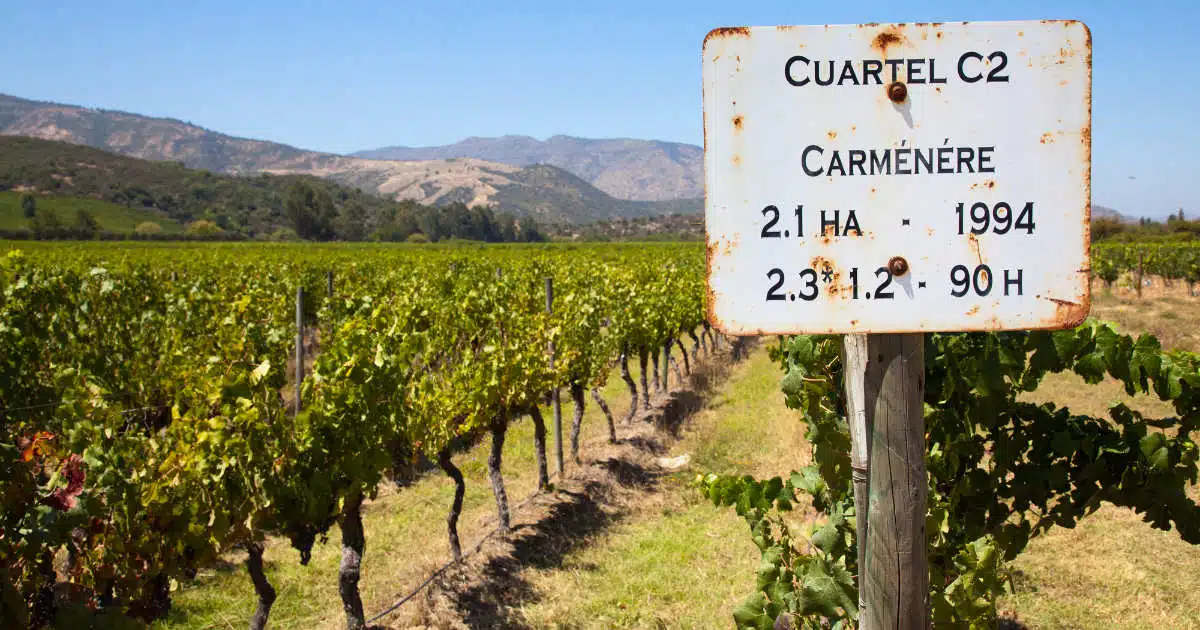
\includegraphics[height=0.7\textheight]{../img/wine.png}  
    \end{figure}
    Motivation: vineyards transporting grapes from harvest site to processing plants
\end{frame}


\begin{frame}{The assigment problem}
    \begin{figure}
        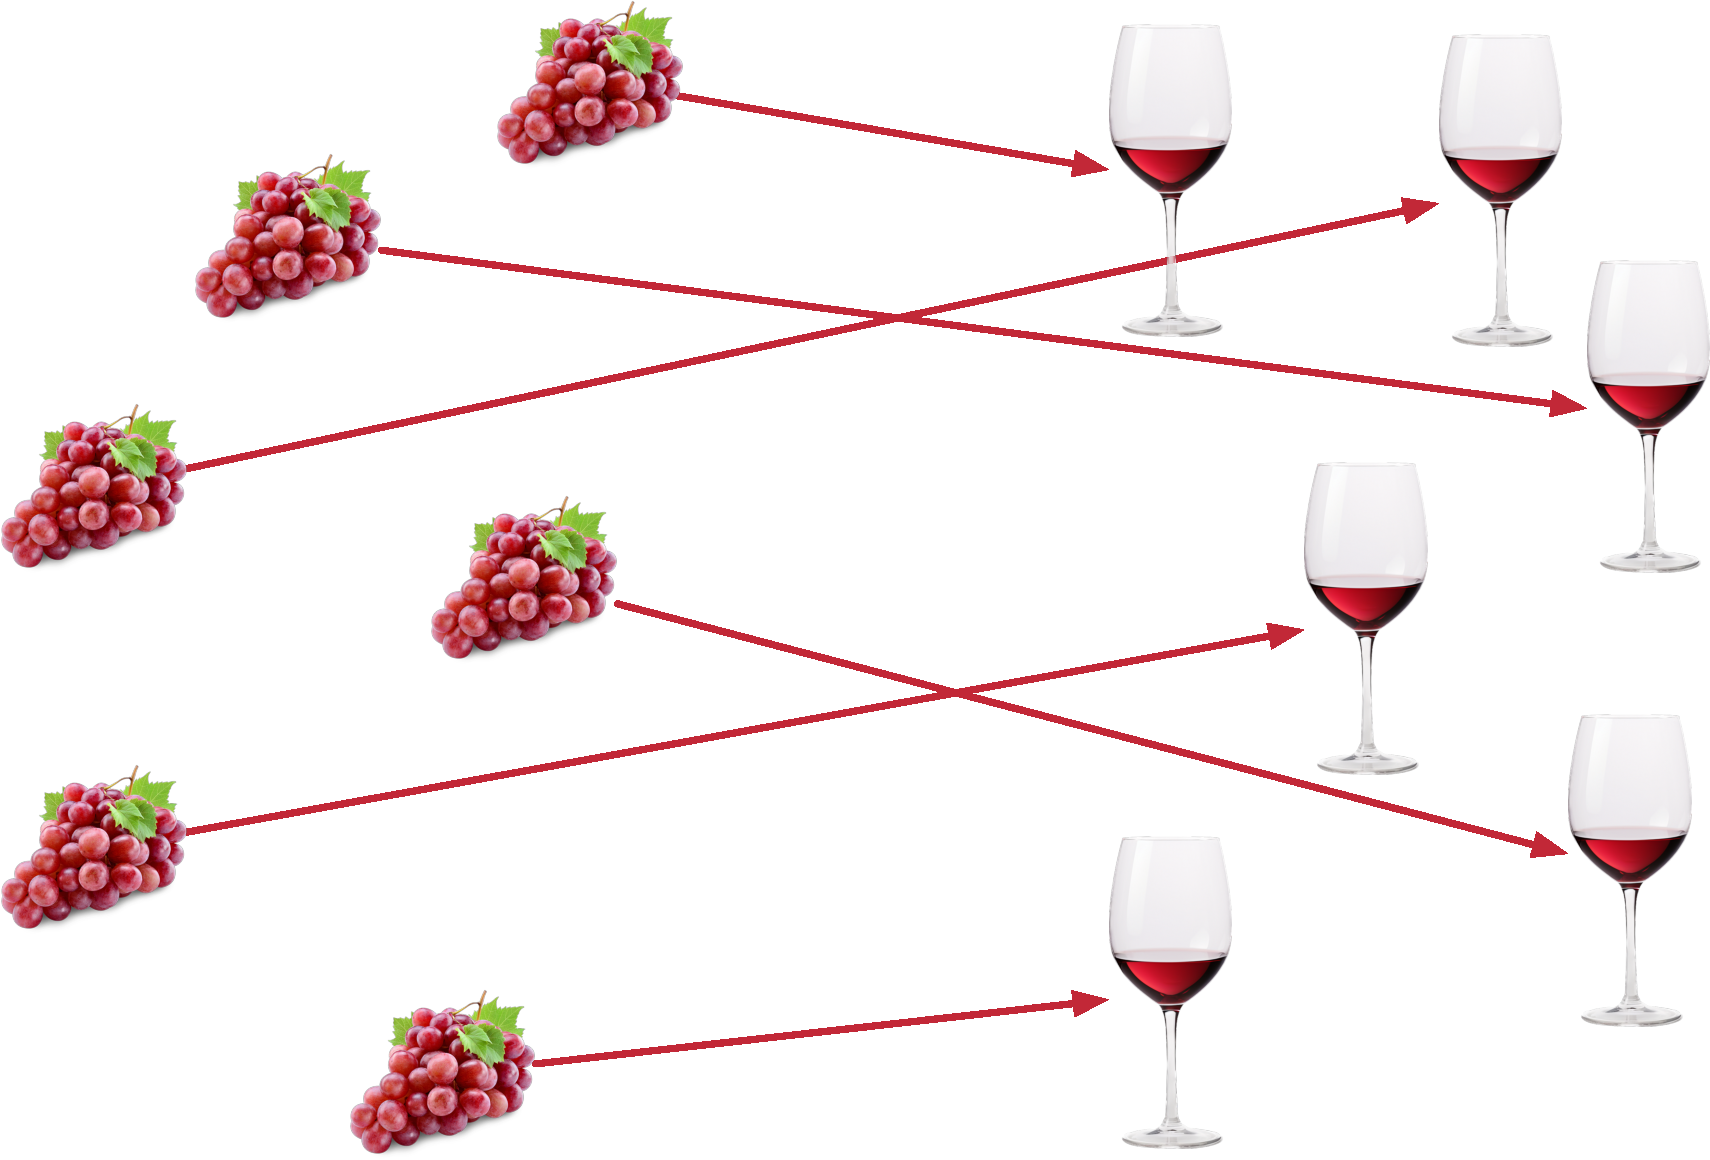
\includegraphics[height=0.7\textheight]{../img/wine_assignment.pdf}  
    \end{figure}
    Build the assignment problem from intuition. Use the above figure to explain all possible ways to assign: straight lines, what's the cost, \emph{cheapest transport}. 
\end{frame}

\begin{frame}{The assigment problem: encoding real-world}

\begin{minipage}{0.45\textwidth}
\begin{itemize}
    \item Weighted masses
    \item Different number of sources/targets
    \item Straight path is not possible
    \item New sample becomes available
\end{itemize}
\end{minipage}
\hfill
\begin{minipage}{0.5\textwidth}
 \begin{figure}
        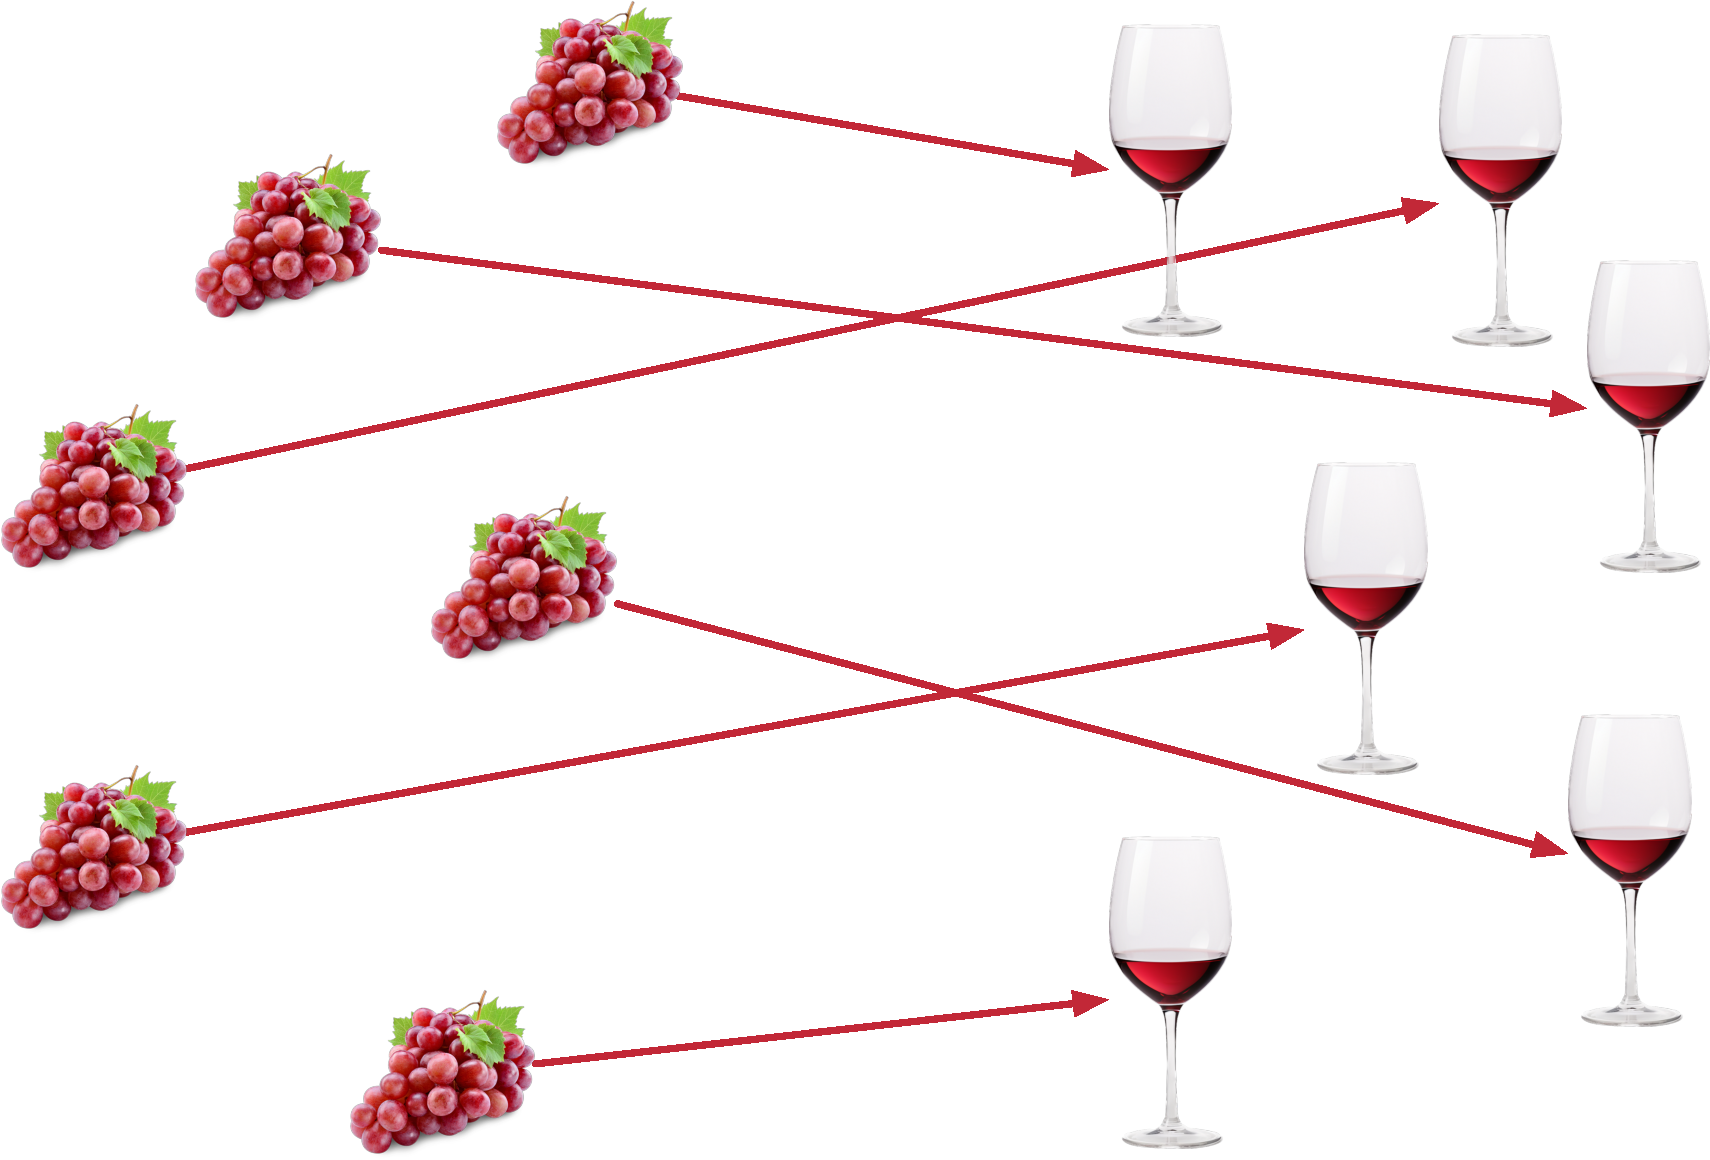
\includegraphics[width=0.99\textwidth]{../img/wine_assignment.pdf}  
    \end{figure}
\end{minipage}

\end{frame}


\begin{frame}[plain]{Monge formulation\footnote{Monge, G. (1781).
Mémoire sur la théorie des déblais et des remblais.
De l'Imprimerie Royale.}}
\bblue{Objective:} Move a pile of mass from one location to another at a minimum effort\\
\vspace{1em}
\bred{Let us first set up our notation} 

\begin{minipage}[t]{0.69\textwidth}

   \begin{itemize}
       \item \bblue{Piles of mass} are probability distributions, $\mu$ and $\nu$, corresponding to random variables $X\in\cX$ and $Y\in\cY$. 
       \item \bblue{Moving procedure} is a function $T: x \in \cX\mapsto Y\in\cY$.
    \item \bblue{Moving cost} encoded as $c: (x,y)\in\cX\times\cY\mapsto c(x,y)\in\R$.
    \item Optimise the total transport cost
    \begin{equation}
        \sum_{x\in\cX} c(x_i, T(x_i))
    \end{equation}
    over $M_{X,Y} = \{ T: \cX \to \cY,\ s.t.,\ T_{\#\mu}=\nu \}$.
   \end{itemize}
\end{minipage}   
\hfill
\begin{minipage}{0.3\textwidth}
       
\end{minipage}   

\end{frame}


\begin{frame}{The transport map (aka the \emph{pushforward} operator $T_\#$)}
    $T$ \emph{transports} mass from $\cX$ to $\cY$, meaning that for any subset $A\in\cY$, one has 
    \begin{equation}
        \nu(A) = \mu(T^{-1}(A)),
    \end{equation}
    where $T^{-1}(A)=\{x\in\cX, s.t.\ T(x)\in A \}$ is the preimage of $A$ under $T$.


\begin{tikzpicture}[>=stealth,scale=1.5]
\small
 \blobA[dashed]{a}{0,0}
  \blobB[dashed]{b}{3,0}
   \node at(0.2,0) {$\XX$};
    \node at(3.2,0) {$\YY$};
  \draw[->] (1.8,1) to[bend left] node[above]{$T$} (3.1,1); 
  \node at(1.5,-0.5) {\footnotesize $A=\{x\in\XX:T(x)\in B\}$};
 \node at(3.55,0) {\scriptsize $B$};
 \draw[->] (0.75,-0.4) to (1.05,-0.05);   
 \node at(6,0.5) {$T\#{\color{red!50} \mu} = {\color{blue!50} \nu}$};
  \node at(6.3,0.2) {i.e., ${\color{red!50} \mu(A)} = {\color{blue!50} \nu(B)}$};
\end{tikzpicture}\\
{\small Figure adapted from Thorpe's book.\footnote{Infinite thanks to Elsa Cazelles (IRIT, CNRS) for kindly sharing these beautiful \texttt{tikz} figures for this part.}}
\end{frame}



\begin{frame}{\bred{Example 1:} Colour transfer}
\begin{minipage}{0.49\textwidth}
\vspace{1em}
\bblue{Original images}
    \begin{figure}
        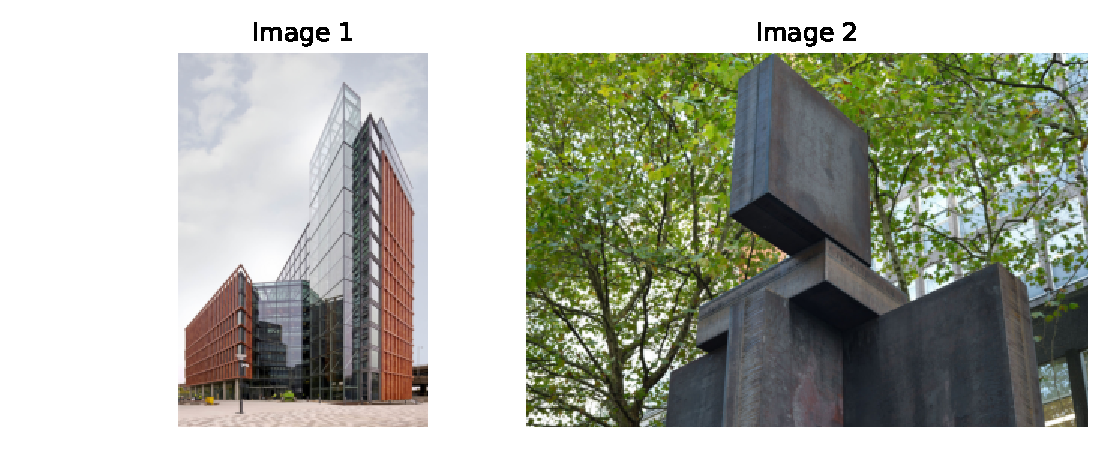
\includegraphics[width=0.9\textwidth]{../img/ex1_original_images.pdf}
    \end{figure}

\bblue{Histograms}
    \begin{figure}
        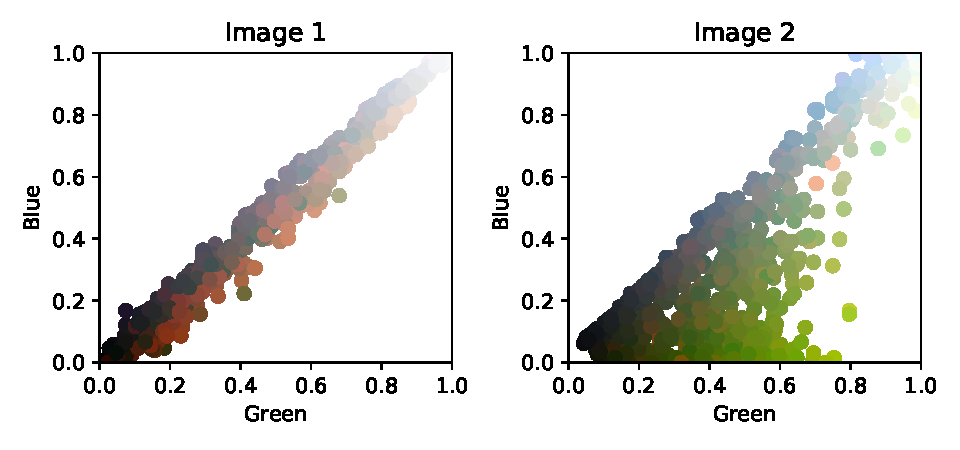
\includegraphics[width=0.9\textwidth]{../img/ex1_colour_histograms.pdf}
    \end{figure}
    
\end{minipage}
\hfill
\begin{minipage}{0.49\textwidth}
\bblue{Histograms}
    \begin{figure}
        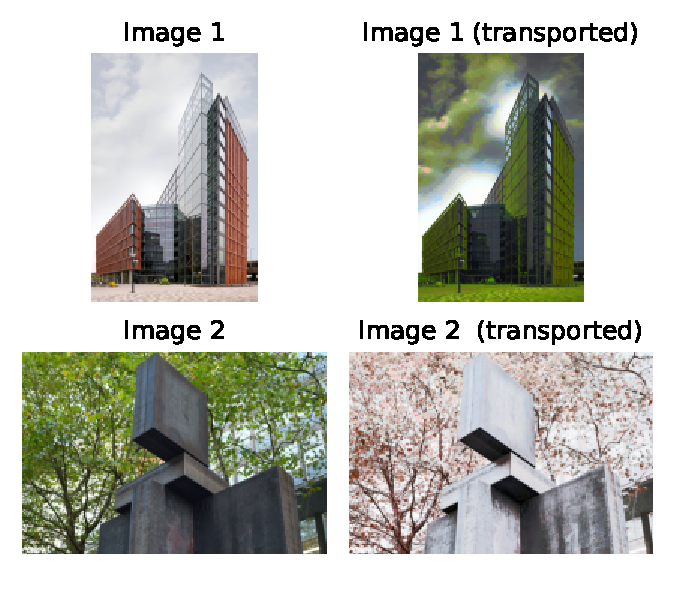
\includegraphics[width=0.9\textwidth]{../img/ex1_result.pdf}
    \end{figure}
\end{minipage}

\begin{textblock}{0.45}(0.56,0.54)
\small
\bred{
\underline{
    Notebook: \href{https://github.com/felipe-tobar/OT-tutorial-MLSP-2024/blob/main/Codes/Colour_transfer.ipynb}{Colour\_transfer.ipynb}
}}
\end{textblock}
\end{frame}


\begin{frame}{\bred{Example 2:} Domain adaptation}

\begin{minipage}{0.49\textwidth}
\vspace{1em}
\bblue{Original images}
    \begin{figure}
        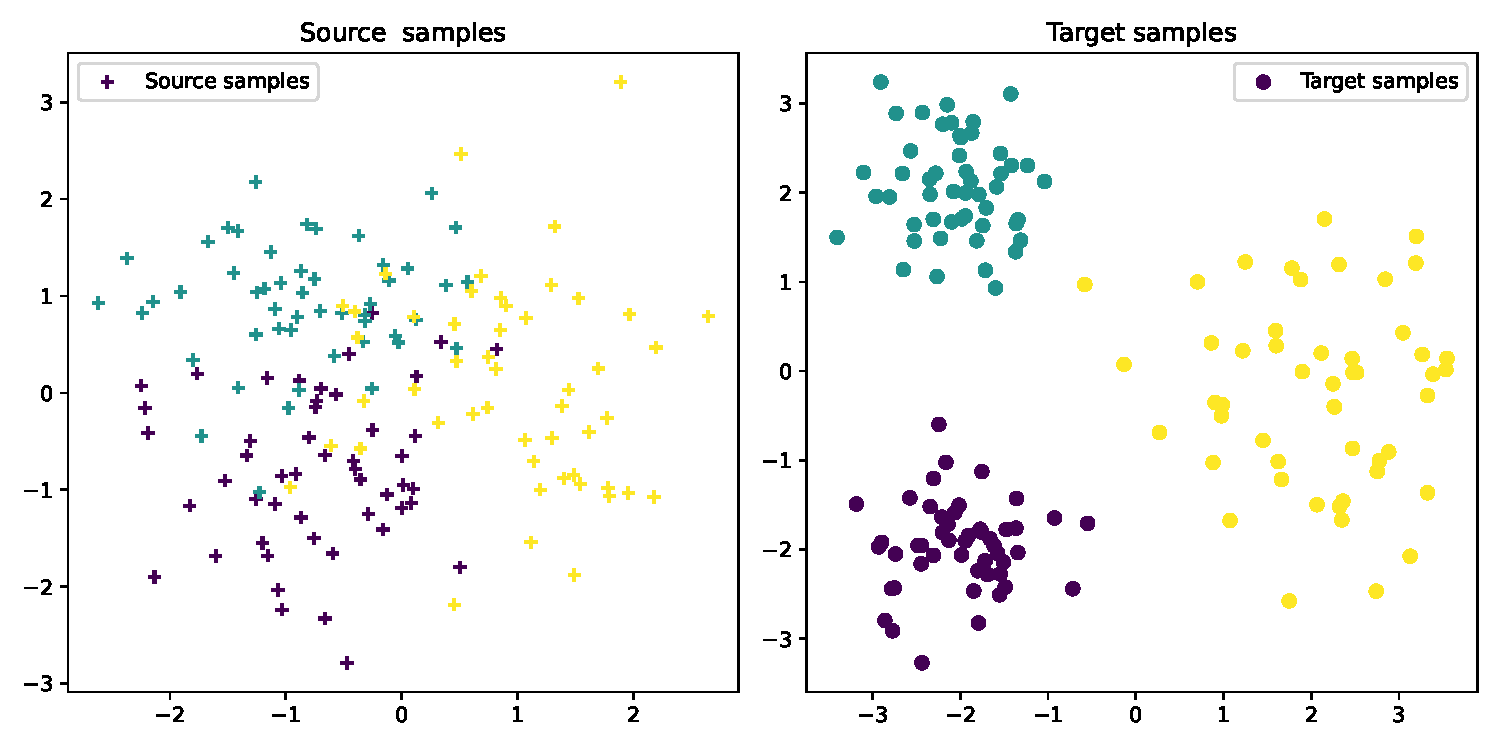
\includegraphics[width=0.78\textwidth]{../img/DA_original_samples.pdf}
    \end{figure}
\vspace{-0.5em}
\bblue{Histograms}
    \begin{figure}
        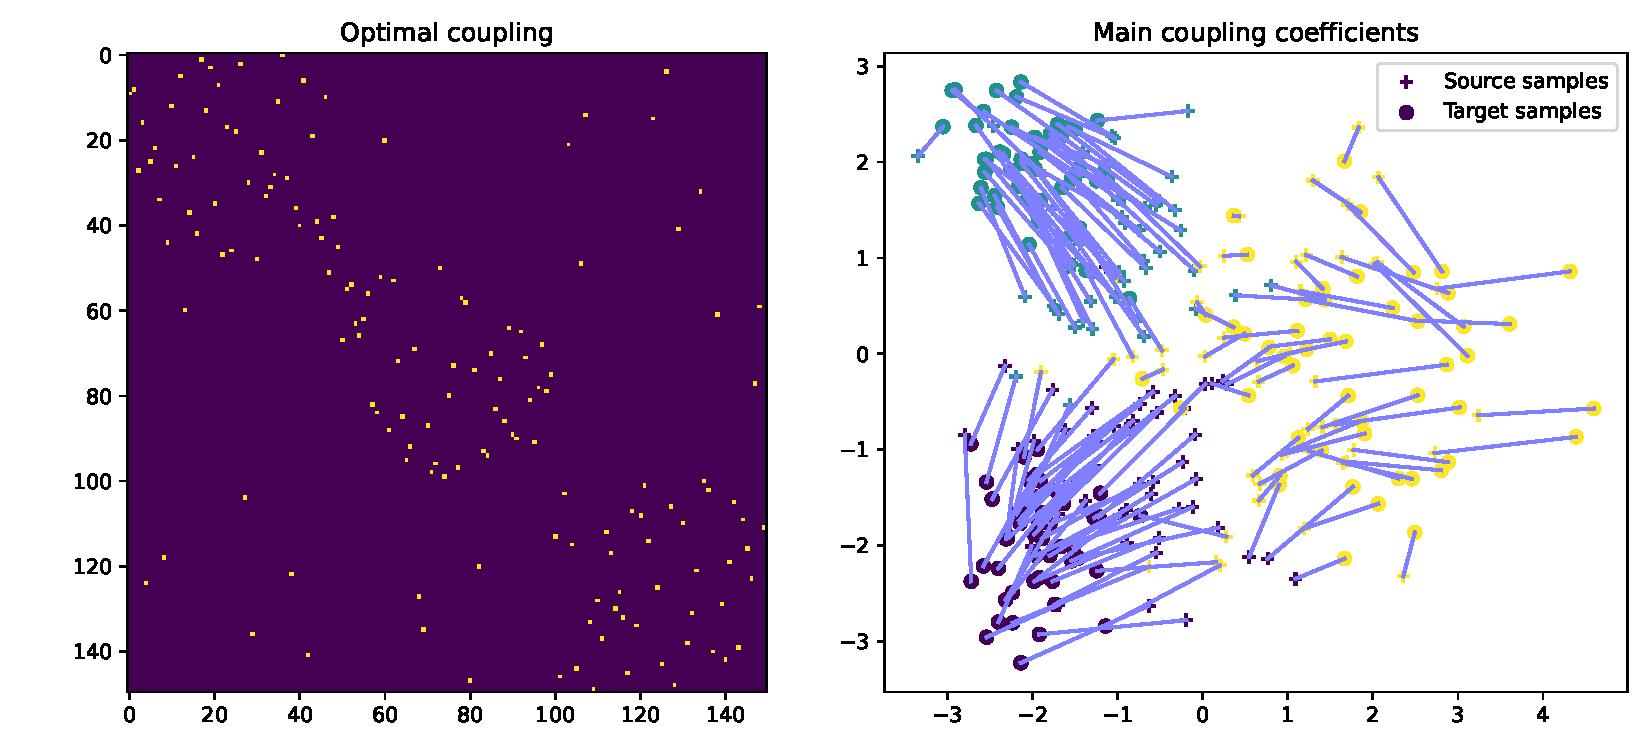
\includegraphics[width=0.85\textwidth]{../img/DA_coupling.pdf}
    \end{figure}
    
\end{minipage}
\hfill
\begin{minipage}{0.49\textwidth}
\bblue{Histograms}
    \begin{figure}
        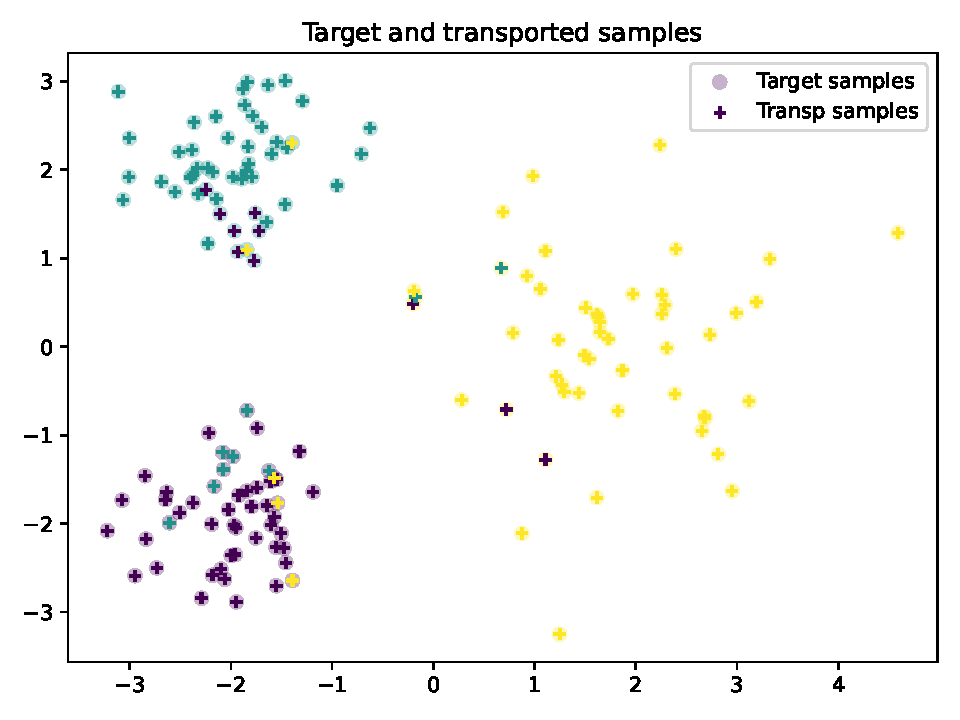
\includegraphics[width=0.9\textwidth]{../img/DA_samples.pdf}
    \end{figure}
\end{minipage}

\begin{textblock}{0.45}(0.56,0.54)
\small
\bred{
\underline{
    Notebook: \href{https://github.com/felipe-tobar/OT-tutorial-MLSP-2024/blob/main/Codes/Domain_adaptation.ipynb}{Domain\_adaptation.ipynb}
}}
\end{textblock}
\end{frame}





\begin{frame}{Neither existence nor uniqueness is guaranteed}
        \begin{figure}
        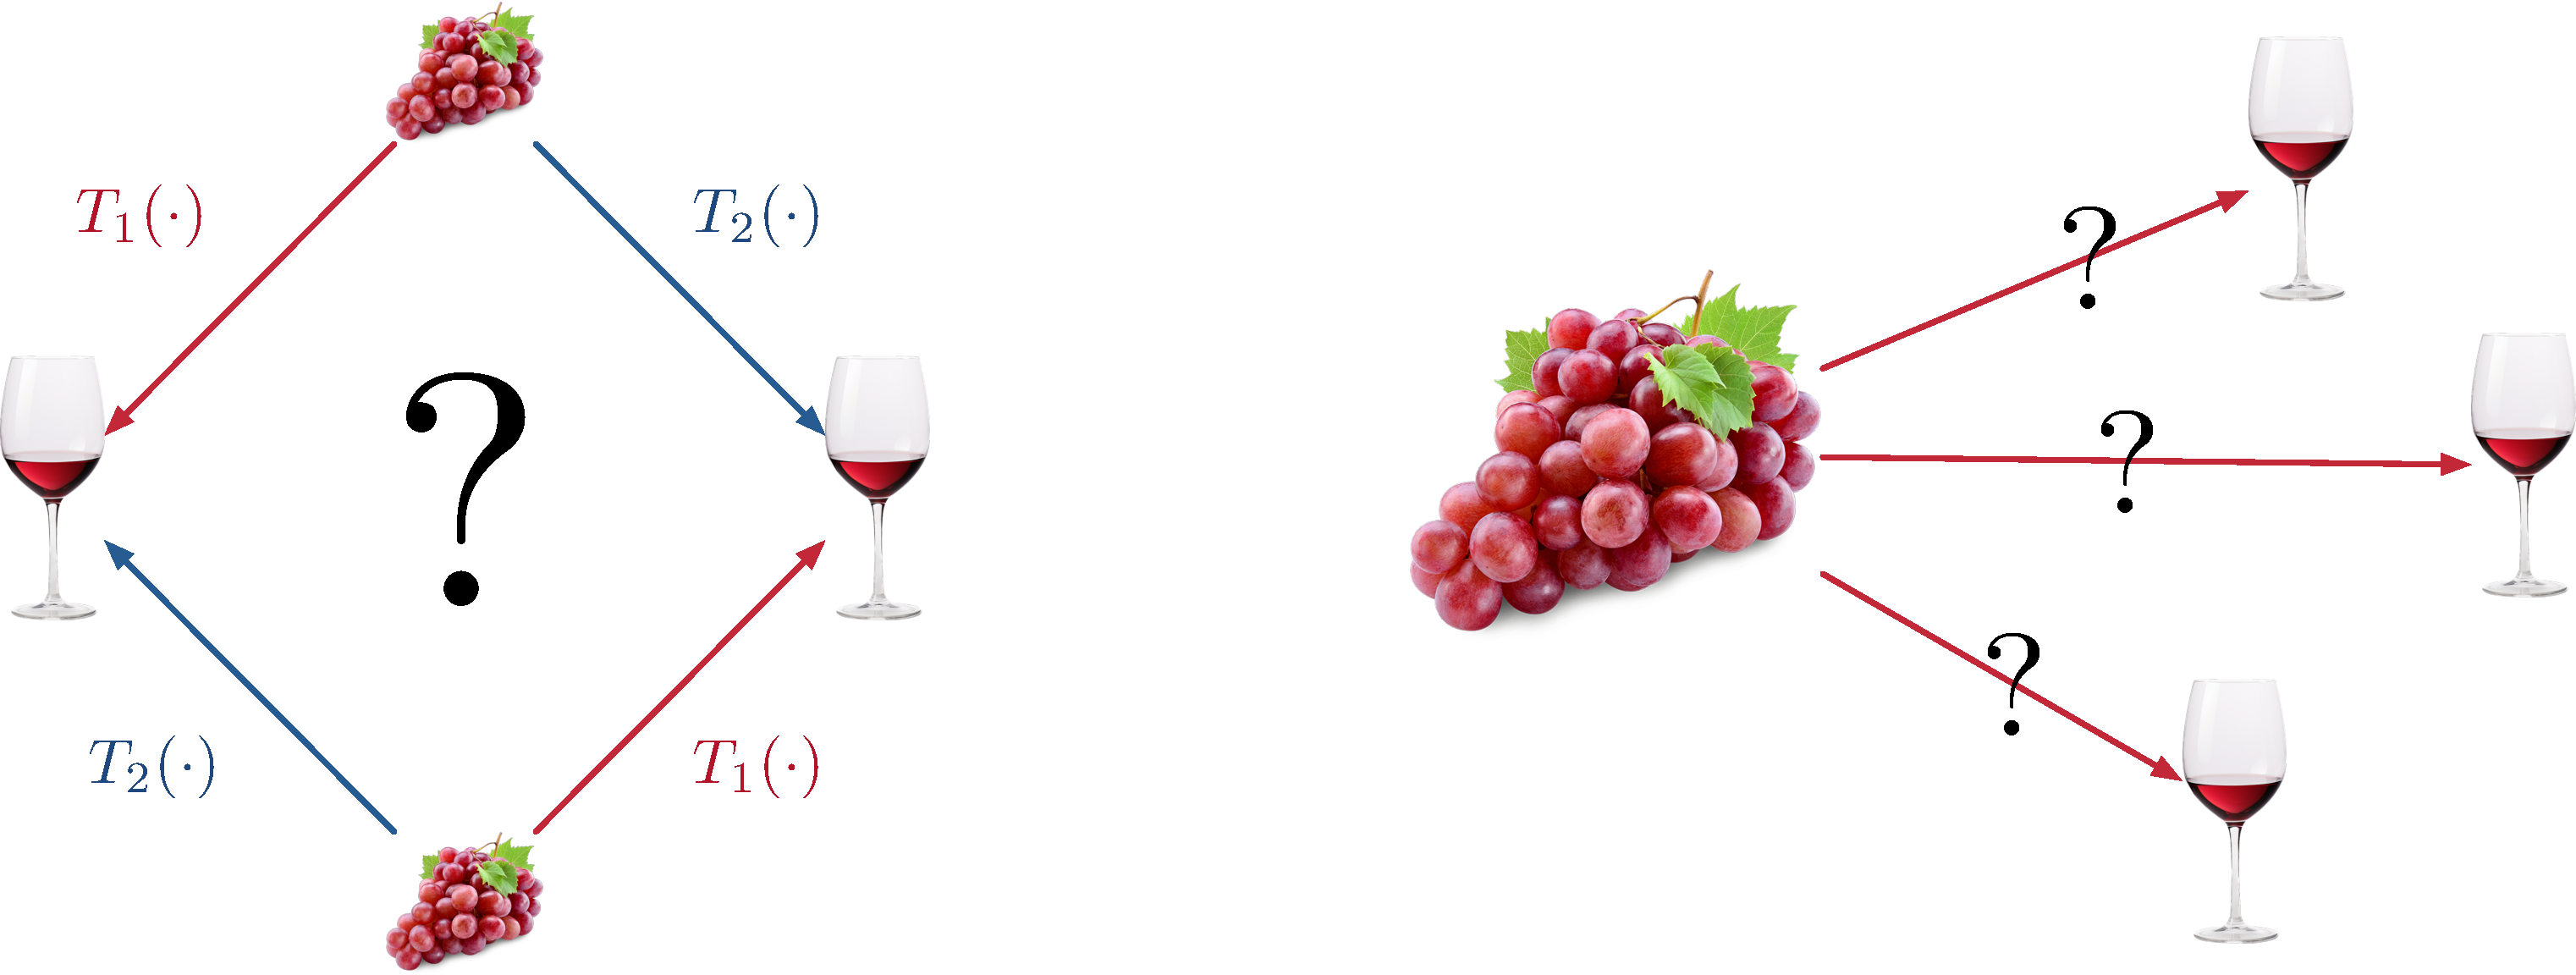
\includegraphics[width=0.7\textwidth]{../img/existence_uniqueness.pdf}
    \end{figure}
    \vspace{1em}
\bred{Observation:} In the above examples, each sample \emph{weighted the same}, i.e., pixels, class instances. In some cases, we might have \emph{weighted samples}.
\end{frame}


\begin{frame}{Kantorovich formulation: mass splitting}

     \begin{figure}
        \includegraphics<1>[width=0.6\textwidth]{../img/wine_assignment.pdf}
        \includegraphics<2>[width=0.6\textwidth]{../img/wine_assignment_split.pdf}
    \end{figure}
\end{frame} 

\begin{frame}{Transport plan} 
\begin{textblock}{0.35}(0.72,0.02)
     \begin{figure}
        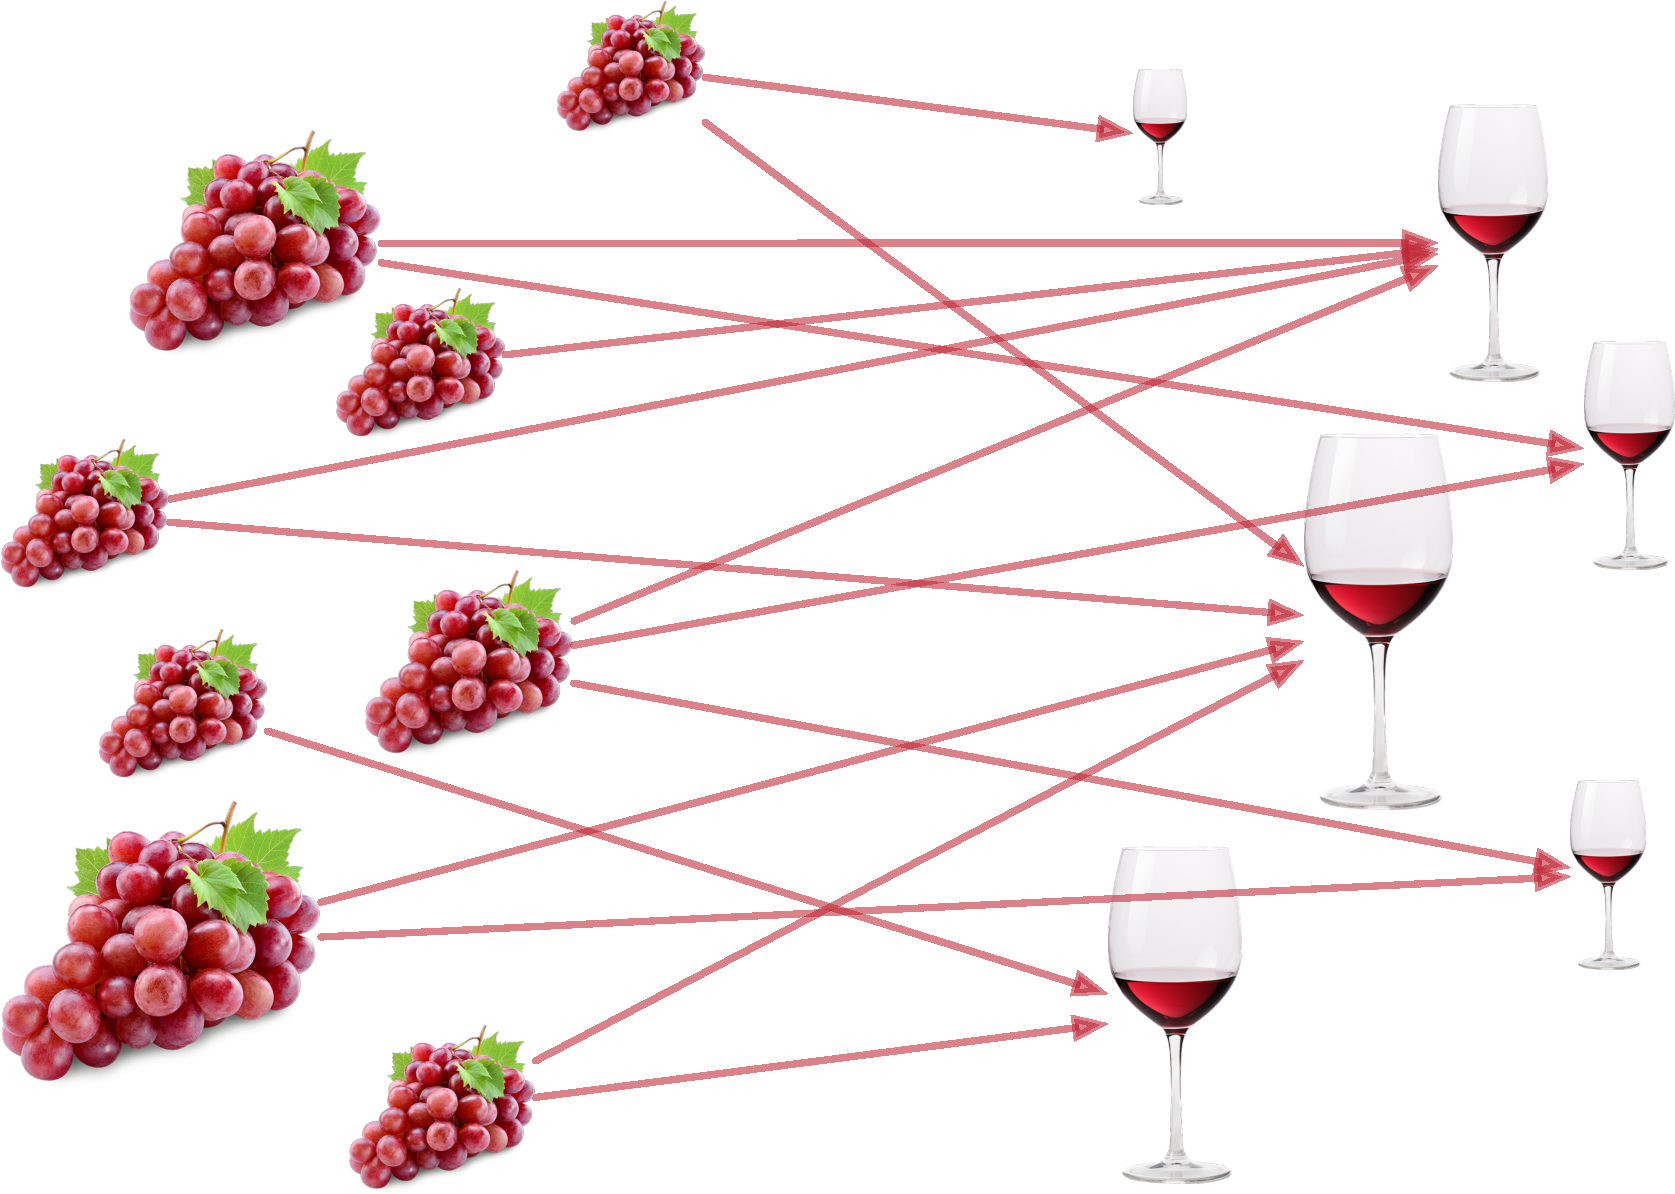
\includegraphics[width=0.6\textwidth]{../img/wine_assignment_split.pdf}
    \end{figure}
\end{textblock}

\begin{equation*}
    \inf_{P\in\Pi_{\mu,\nu}} \langle P , C\rangle = \sum_{i,j}^{n,m} C_{ij}P_{ij} 
\end{equation*}
where $\Pi_{\mu,\nu} \langle P , C\rangle = \{  P\in [0,1]^{m\times n} :  \sum_{i=1}^m P_{ij} = \nu_j,  \sum_{j=1}^n P_{ij} = \mu_i \}$
    \begin{figure}
        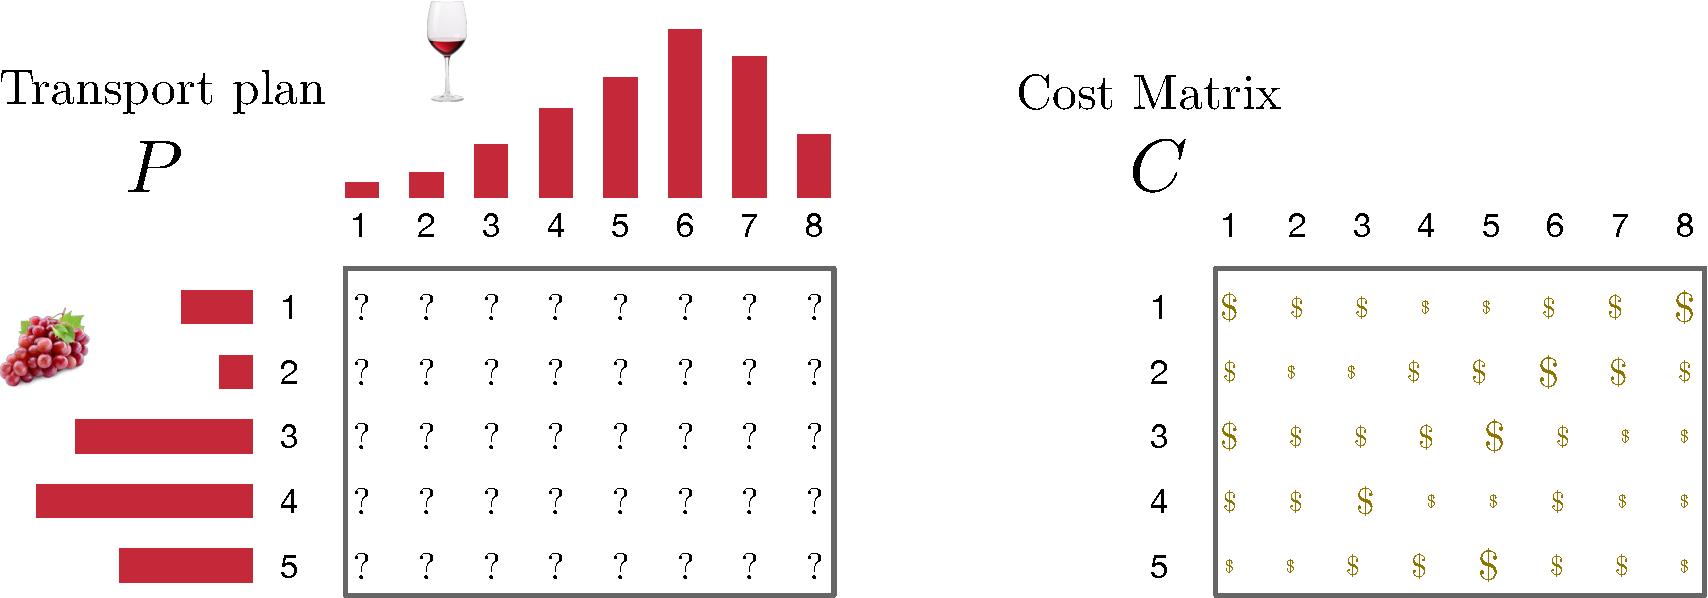
\includegraphics[width=0.9\textwidth]{../img/kantorovich.pdf}
    \end{figure}
\end{frame}



\begin{frame}{\bred{Example 3:} Discrete Kantorovich plan}
    Let consider the following source and target distributions

\begin{minipage}{0.49\textwidth}
\begin{figure}
        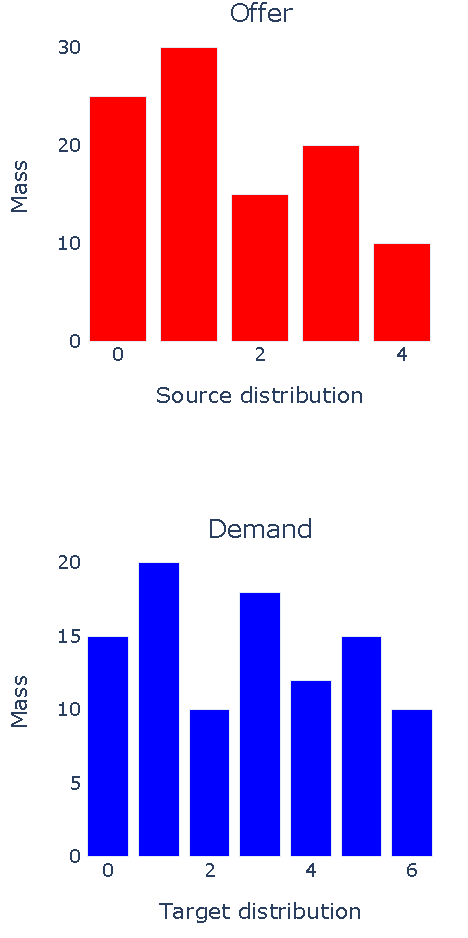
\includegraphics[width=0.48\textwidth]{../img/kantorovich_discrete_histogram.pdf}\hspace{2em}
    \end{figure}
\end{minipage}
\hfill
\begin{minipage}{0.49\textwidth}
\begin{figure}
        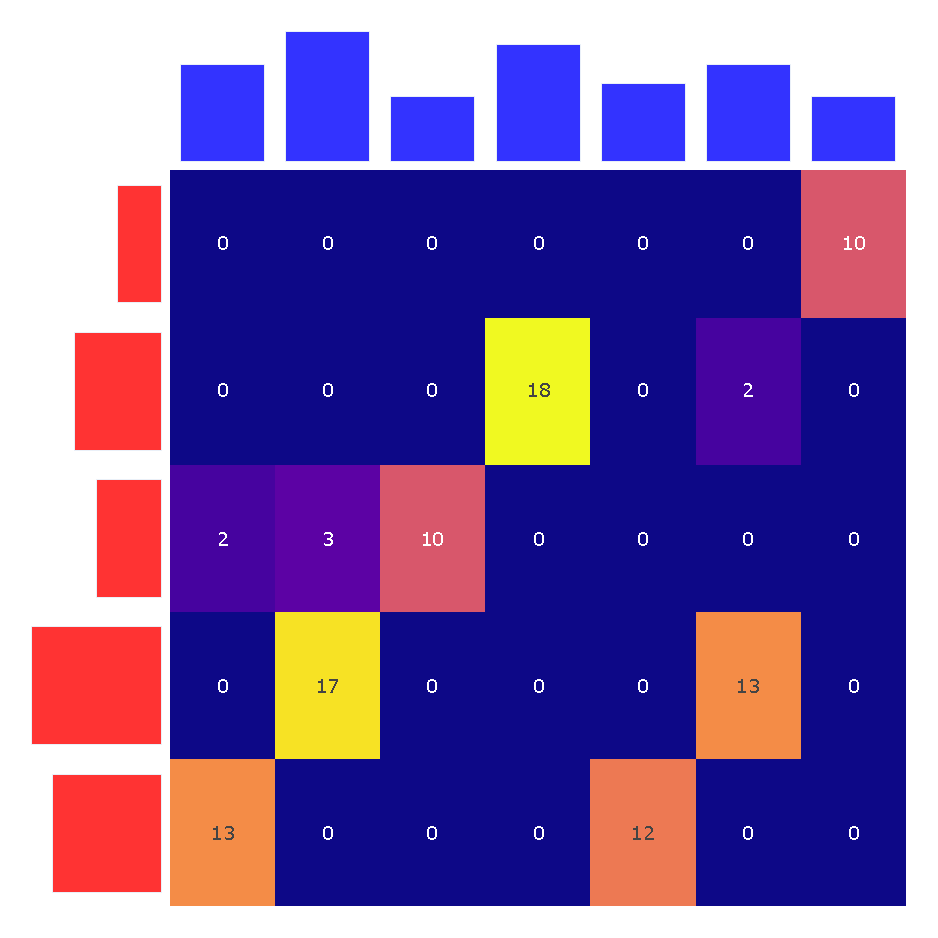
\includegraphics[width=0.8\textwidth]{../img/kantorovich_discrete_solution.pdf}\hspace{2em}
    \end{figure}
\end{minipage}

\begin{textblock}{0.45}(0.62,0.54)
\small
\bred{
\underline{
    Notebook: \href{https://github.com/felipe-tobar/OT-tutorial-MLSP-2024/blob/main/Codes/kantorovich.ipynb}{kantorovich.ipynb}
}}
\end{textblock}
\end{frame}




\begin{frame}{\bred{Example 4:} Continuous Kantorovich plan}
    Let us now consider two  distributions over a continuous support
\begin{minipage}{0.59\textwidth}
\begin{figure}
    \centering
        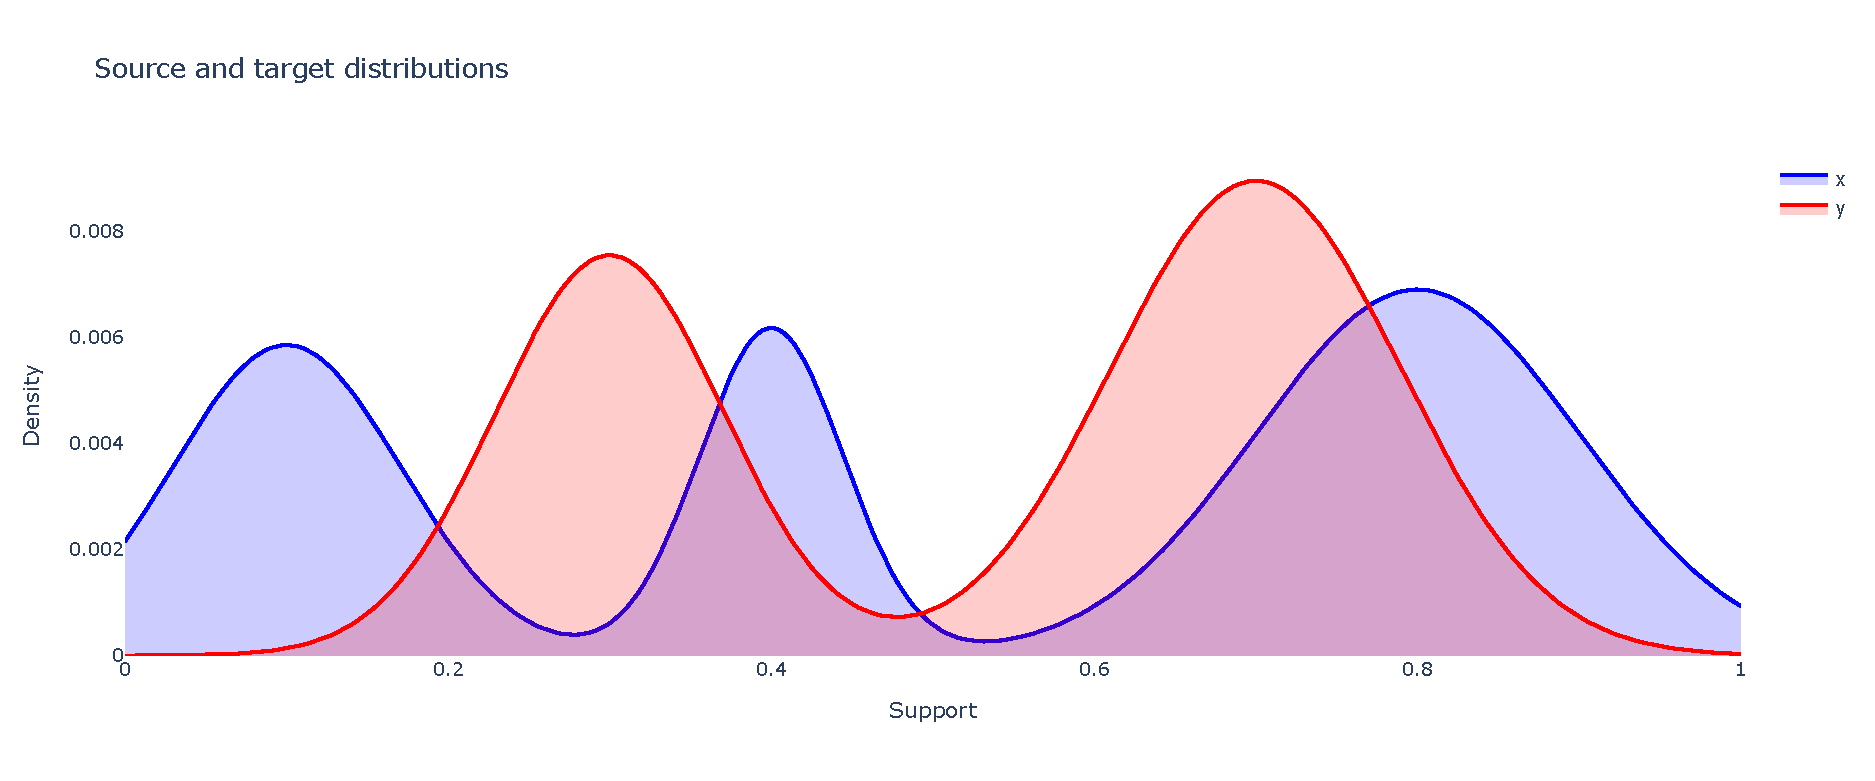
\includegraphics[width=0.9\textwidth]{../img/kantorovich_continuous_density.pdf}\hspace{2em}
    \end{figure}
            \bblue{Observe that the plan remained \emph{sparse}, i.e., the mass did not spread  much}

        This motivates the following results
\end{minipage}
\hfill
\begin{minipage}{0.4\textwidth}
\begin{figure}
    \centering
        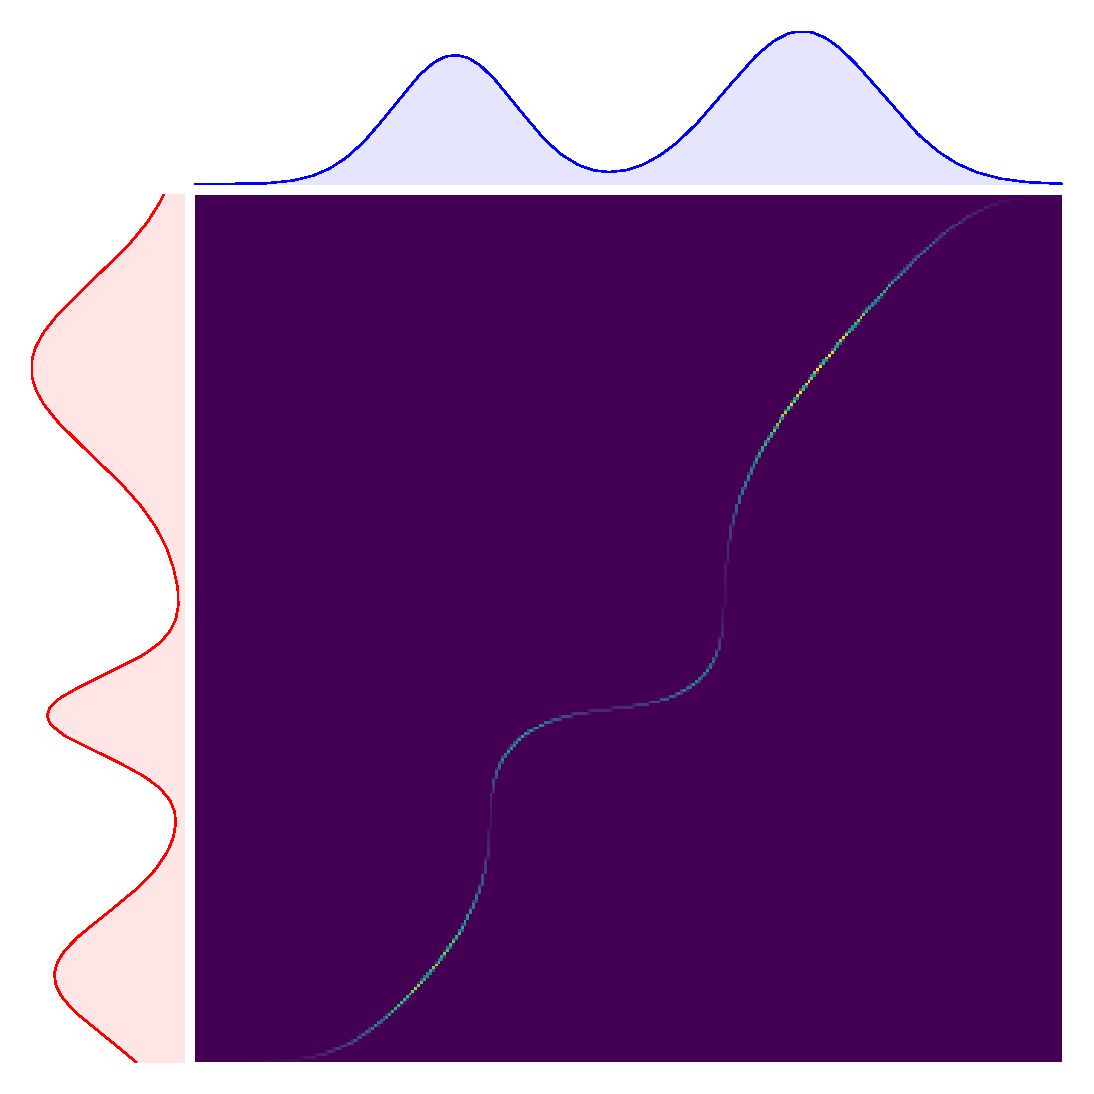
\includegraphics[width=0.9\textwidth]{../img/kantorovich_continuous_solution.pdf}
    \end{figure}
    \centering
    \small
\bred{
\underline{
    Notebook: \href{https://github.com/felipe-tobar/OT-tutorial-MLSP-2024/blob/main/Codes/kantorovich.ipynb}{kantorovich.ipynb}
}}
\end{minipage}
\end{frame}


\begin{frame}{Observations}
    \begin{itemize}
        \item Let us consider a cost $c(x,y) = |x-y|^p, p\geq 1$. Then, if $\mu$ and $\nu$ are absolutely continuous wrt the Lebesgue measure, the Kantorovich problem as a unique solution. Furthermore, this solution is the same solution of the Monge problem.
        \item If $p=2$, the optimal map is the gradient of a convex function
        \item In some cases the optimal plan will require to split mass (e.g., in the case of atomic measures) and thus Monge's solution may fail to exist. 
        \item Luckily, from a (Kantorovich) transport plan we can always extract a tranport map, e.g., via the barycentric projection
    \end{itemize}
\end{frame}






\begin{frame}{Dual formulation}
    Formualtion and illustration with the factories
\end{frame}

\begin{frame}{\bred{Example 5:} Wasserstein GANs}
diagrams, figures and hopefully code
\end{frame}


\section{Part II: Metric properties}



\begin{frame}{Motivation}
    We need a distance, OT provides one. Show how some \emph{strong} topologies cannot be used for learning systems
\end{frame}

\begin{frame}{The Wasserstein distance}
    Definition, properties
\end{frame}

\begin{frame}{The Wasserstein space}
    Definition, properties
\end{frame}

\begin{frame}{Convergence properties, weak topology}
    Revise the above example
\end{frame}


\begin{frame}{Geodesic properties}
    Interpolation
\end{frame}

\begin{frame}{The Wasserstein barycenter}
    Definition, properties, example
\end{frame}


\begin{frame}{Examples}
    See which ones make sense here:  OT spectral transport, Wasserstein Bays, VAEs.
\end{frame}


\section{Closing remarks}

\begin{frame}{What we did not see}
   multimarginal, unbalanced OT, partial OT, Gromov-Wasserstein, 
\end{frame}


\begin{frame}{Conclusions \& the future}
\end{frame}






\begin{frame}[plain]
    \titlepage
\end{frame}





\end{document}